% Sources : 
%    * http://tex.stackexchange.com/questions/83727/pretty-lists-for-sorting-algorithms
%    * http://tex.stackexchange.com/questions/94120/tikz-arrows-for-displaying-sorting-algorithms/94124#94124

\documentclass{article}
    \usepackage{tikz}
    \usepackage{xstring}
    \usetikzlibrary{calc,positioning}
    \tikzset{
        raw sort entry/.style = {
            rectangle, thick, draw, node distance = 1.5em
        },
        sort entry black/.style = {
            raw sort entry, black,  fill = white
        },
        sort entry blackgray/.style = {
            raw sort entry, black,  fill = gray!25
        },
        s1/.style = {
            raw sort entry, red,    fill = yellow!30
        },
        s2/.style = {
            raw sort entry, blue,   fill = green!20
        },
        s3/.style = {
            raw sort entry, violet, fill = orange!25
        },
        /qrr/default/.style = sort entry black,
        name row/.initial = {},
        previous row/.initial = {},
        previous col/.initial = {1},
        default/.style = {/qrr/default/.style = {#1}},
        |-|/.style = {
            to path = {
                let \p1 = (\tikztostart),
                    \p2 = (\tikztotarget) in
                        -- (\x1,.5*\y1+.5*\y2)
                        -- (\x2,.5*\y1+.5*\y2) \tikztonodes
                        -- (\tikztotarget)
            }
        }
    }

    \newcommand*{\List}[2][default = sort entry black]{%
        \tikzset{#1}%
        \edef\listtoprocess{#2}%
        \pgfkeysgetvalue{/tikz/name row}{\rowname}%
        \pgfkeysgetvalue{/tikz/previous row}{\previousRow}%
        \pgfkeysgetvalue{/tikz/previous col}{\previousCol}%
        \def\ListToProcess{}%
        \foreach \content in \listtoprocess{
            \IfSubStr{\content}{/}{% true
                \xdef\ListToProcess{\ListToProcess,\content}
        }{%                            false
            \xdef\ListToProcess{\ListToProcess,{/qrr/default}/\content}
        }
    }

    \StrGobbleLeft{\ListToProcess}{1}[\ListToProcess]%
% Removes the first comma (\listToProcess is empty at the start)
        \foreach [count = \i] \Style/\Value in \ListToProcess {
            \ifnum\i = 1\relax
                \expandafter\ifx\expandafter\relax\previousRow\relax
                \node [raw sort entry, \Style] (\rowname-\i) {\Value};
            \else
                \node [raw sort entry, \Style, below = 1em of \previousRow-\previousCol] (\rowname-\i) {\Value};
            \fi
            \else
                \node [raw sort entry, right = .5em of \rowname-\number\numexpr\i-1\relax, \Style] (\rowname-\i) {\Value};
            \fi
      }
      \tikzset{previous row/.expand once = \rowname}
    }

\begin{document}

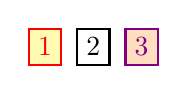
\begin{tikzpicture}
    \List{s1/1, 2, s3/3}
\end{tikzpicture}

\bigskip

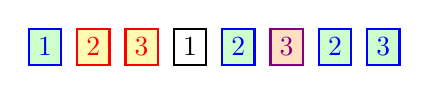
\begin{tikzpicture}
    \List[sort entry blackgray]{
        s2/1, s1/2, s1/3, 1, s2/2, s3/3, s2/2, s2/3
    }
\end{tikzpicture}


\bigskip


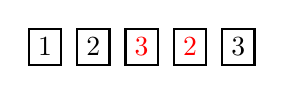
\begin{tikzpicture}
    \List[s1]{1, 2, /3, /2, 3}
% /3 and /2 falls back to no explicit \Style, so the resulting
% style is that from the \node [raw sort entry, …]
\end{tikzpicture}


\bigskip


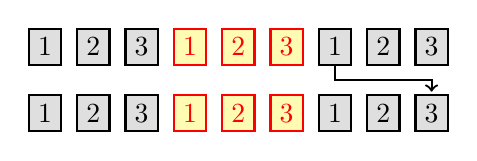
\begin{tikzpicture}
    \List[
        default  = sort entry blackgray,
        name row = a]{
        1, 2, 3, s1/1, s1/2, s1/3, 1, 2, 3
    }

    \List[default = sort entry blackgray, name row = b]{
        1, 2, 3, s1/1, s1/2, s1/3, 1, 2, 3
    }

    \draw[thick, shorten > = \pgflinewidth,->] (a-7) to[|-|] (b-9);
\end{tikzpicture}


\bigskip


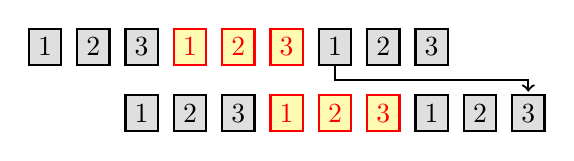
\begin{tikzpicture}
    \List[
        default  = sort entry blackgray,
        name row = a
    ]{
        1, 2, 3, s1/1, s1/2, s1/3, 1, 2, 3
    }

    \List[
        default  = sort entry blackgray,
        name row = b, previous row = a, previous col = 3
    ]{
        1, 2, 3, s1/1, s1/2, s1/3, 1, 2, 3
    }

    \draw[thick, shorten > = \pgflinewidth,->] (a-7) to[|-|] (b-9);
\end{tikzpicture}

\end{document}